\chapter{Proof of Concept}
Nun wird das realisierte Konzept anhand der in Kapitel~\ref{scenarios} vorgestellten Fallstudien auf Applikabilität geprüft.
Aus den Ergebnissen dieses Kapitels kann im Anschluss ein Fazit gezogen und ein potenzieller Ausblick auf künftige Erweiterungen des Konzepts gegeben werden.

\section{Von 3D Gebäudeplan zu Bauplanentwurf}
Zunächst müssen für einzelnen Szenarien der ersten Fallstudie Gebäudepläne in einem Konstruktionsplaner modelliert werden.
Dazu wurde, wie schon in Kapitel~\ref{real:modellierung} beschrieben, die 3D Modellierungs-Software Blender herangezogen (siehe Kapitel~\ref{basics:blender}).
Diese kann mit der frei verfügbaren Erweiterung \textit{blenderbim} zu einem funktionsfähigen BIM Editor mit \textit{IFC} Unterstützung ausgebaut werden.
Auch diese Technologien wurden bereits in den Kapiteln~\ref{basics:blenderbim} und~\ref{basics:ifc} vorgestellt.
Darin können sowohl individuelle Wandtypen definiert, als auch Annotationen über Modul und Rastermaß mithilfe eigener \textit{IfcPropertySets} daran angehängt werden.
Mit den in Kapitel~\ref{concept:raster} definierten Modellierungseinschränkungen, deren Umsetzung in Kapitel~\ref{real:modellierung} thematisiert wurde, konnte die Modellierungsphase sowohl erleichtert, als auch beschleunigt werden.

\subsection{Szenario Turm}\label{poc:scenario1}
\begin{figure}[hbt]
  \hspace*{\fill}%
  \begin{subfigure}[b]{0.25\columnwidth}
    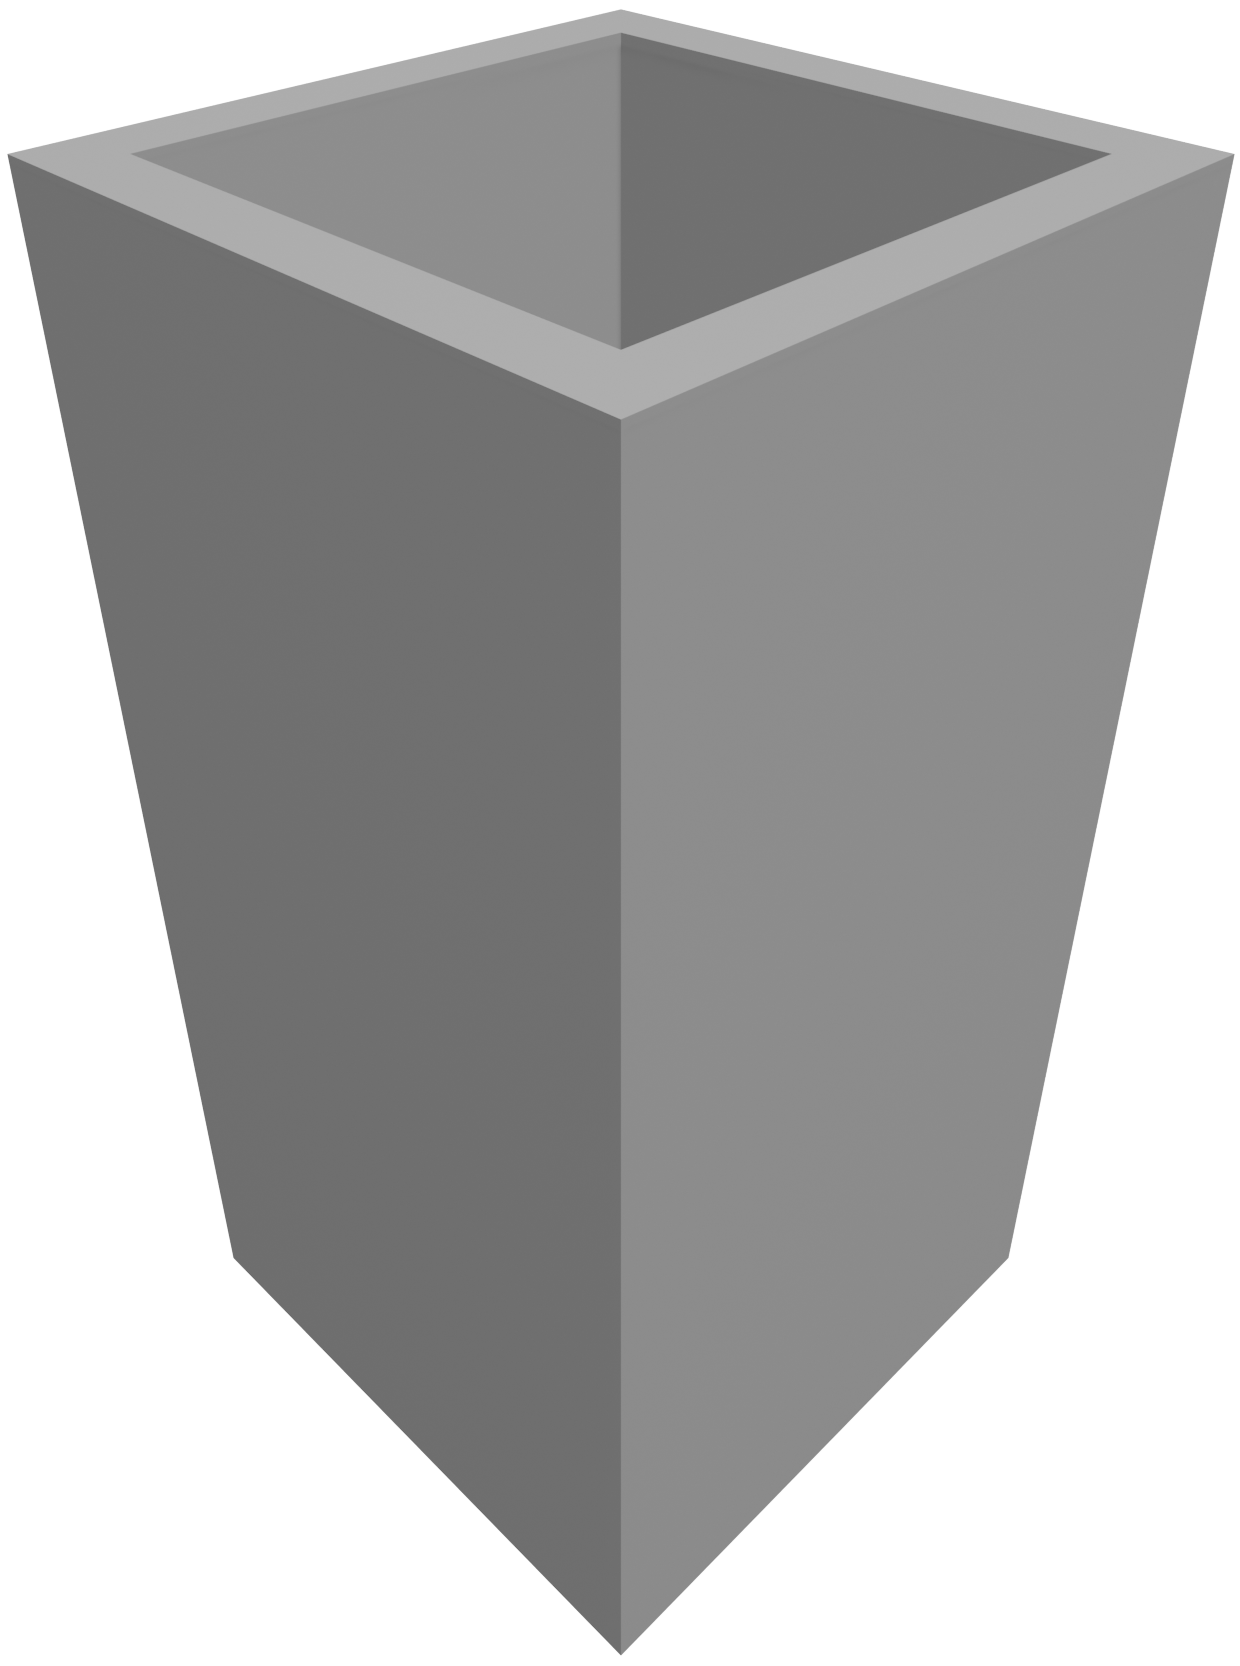
\includegraphics[width=\columnwidth]{fig/scenario1_render_base_thin.png}
    \caption{Der Turm mit 1 Meter dicken Wänden.}\label{fig:poc:scenario1_wall_thin}
  \end{subfigure}
  \hfill%
  \begin{subfigure}[b]{0.25\columnwidth}
    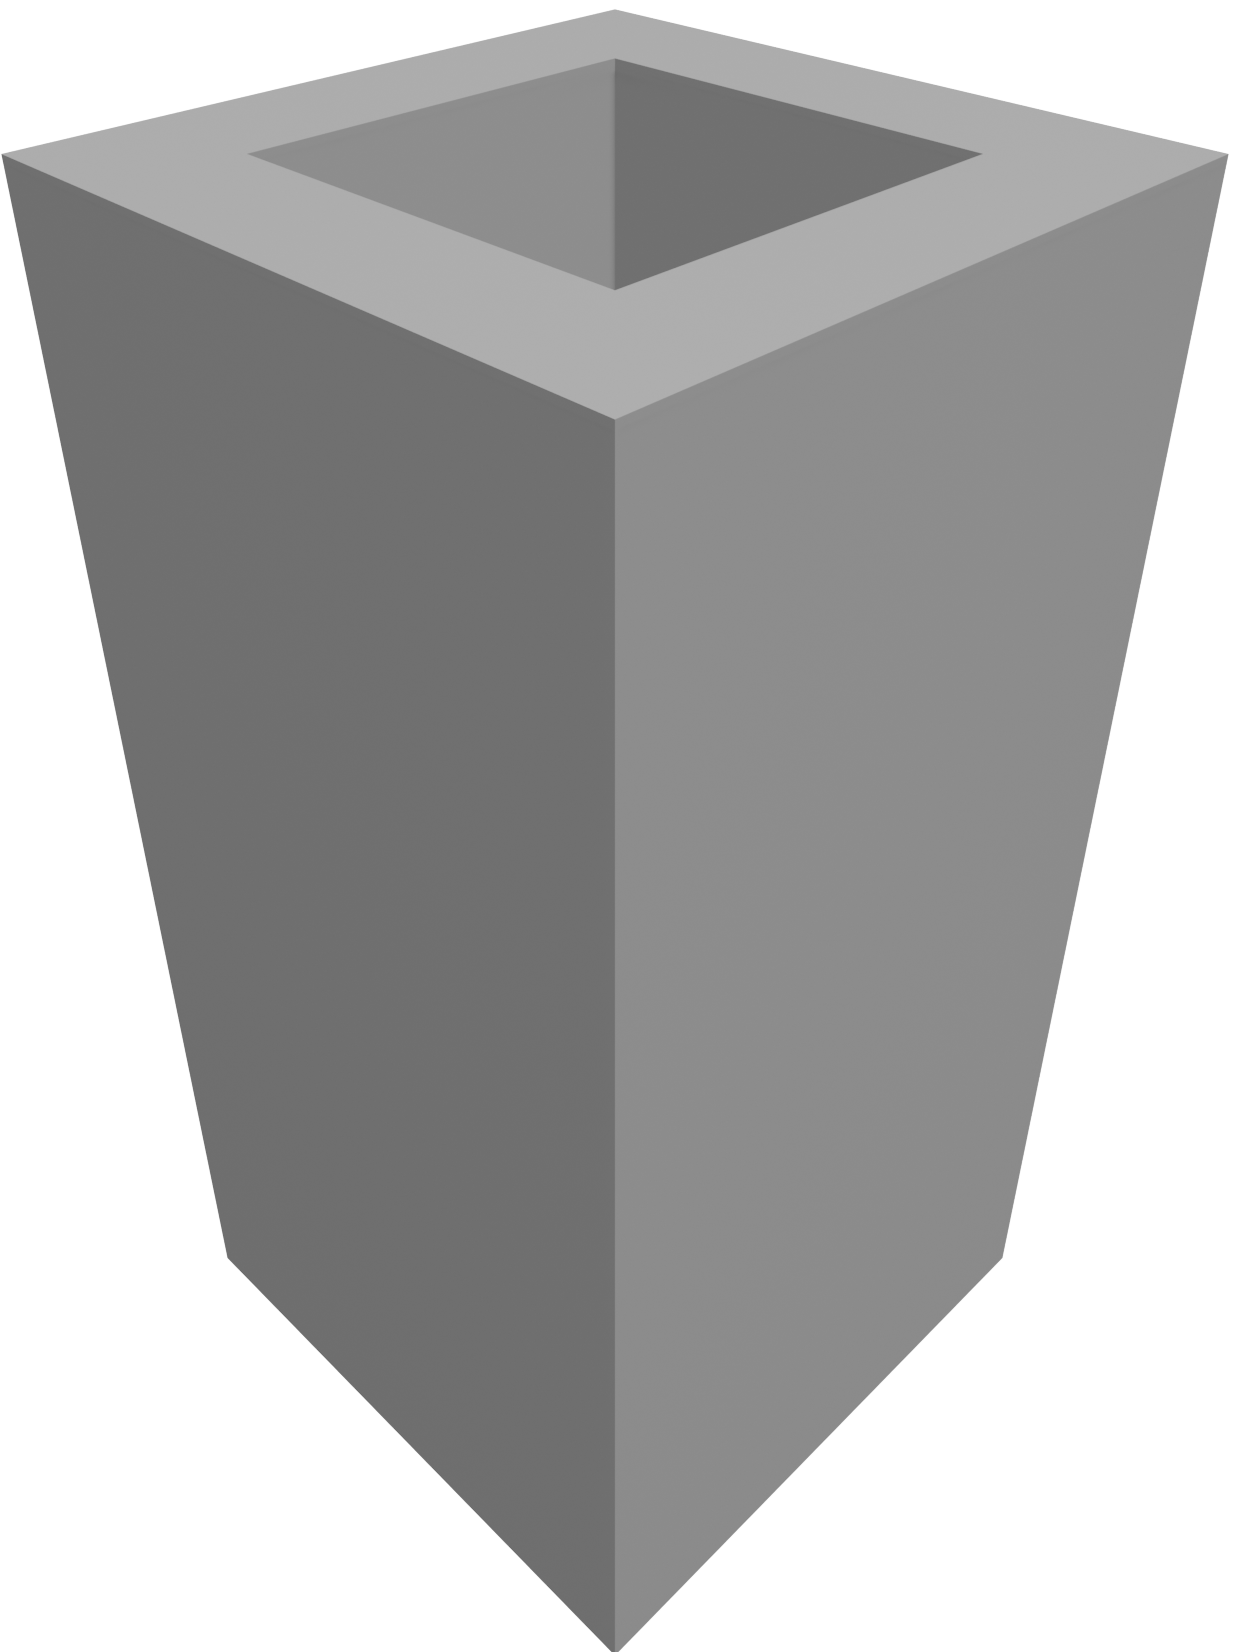
\includegraphics[width=\columnwidth]{fig/scenario1_render_base_thick.png}
    \caption{Der Turm mit 2 Meter dicken Wänden.}\label{fig:poc:scenario1_wall_thick}
  \end{subfigure}
  \hspace*{\fill}%
  \caption{Die beiden Eingabemodelle des Turmes im IFC Format.}\label{fig:poc:scenario1 modell}
\end{figure}
Die Modellierung der zwei sich in der Wanddicke unterscheidenden Versionen des 20 Meter hohen Turms mit einer Grundfläche von 10$\times$10 Metern in Blender war wenig komplex.
Es bedarf lediglich vier Wände, die einen quadratischen Raum bilden.
Die vollständigen Gebäudemodelle sind in Abbildung~\ref{fig:poc:scenario1 modell} zu sehen.
Das Ergebnis nach Anwenden der drei verschiedenen Mauerwerksverbände ist wie erwartet.
Die verschiedenen Verbände lassen sich, wie in Kapitel~\ref{real:verband} gezeigt, in den Programmcode einpflegen.
Das Basismodul ist überall dort zu sehen, wo ein gerader Wandabschnitt vorliegt.
Alle vier Eckbereiche sind korrekt identifiziert worden, denn dort wurde der für den jeweiligen Mauerwerksverband vordefinierte Eckplan passend umgesetzt.
Im Falle des Kreuz- und Kopfverbandes wurde das Basismodul dabei etwas verkürzt.
Die drei den Bauplanentwürfe werden als JSON-Dateien ausgegeben.
Darin sind alle in Abschnitt~\ref{real:export} angegebenen Informationen enthalten.
In Abbildung~\ref{fig:poc:result_scenario1} sind die ebenfalls exportierten Meshes der drei mit Bausteinen realisierten Türme zu sehen.

\begin{figure}[htb]
    \begin{subfigure}[b]{0.3\columnwidth}
      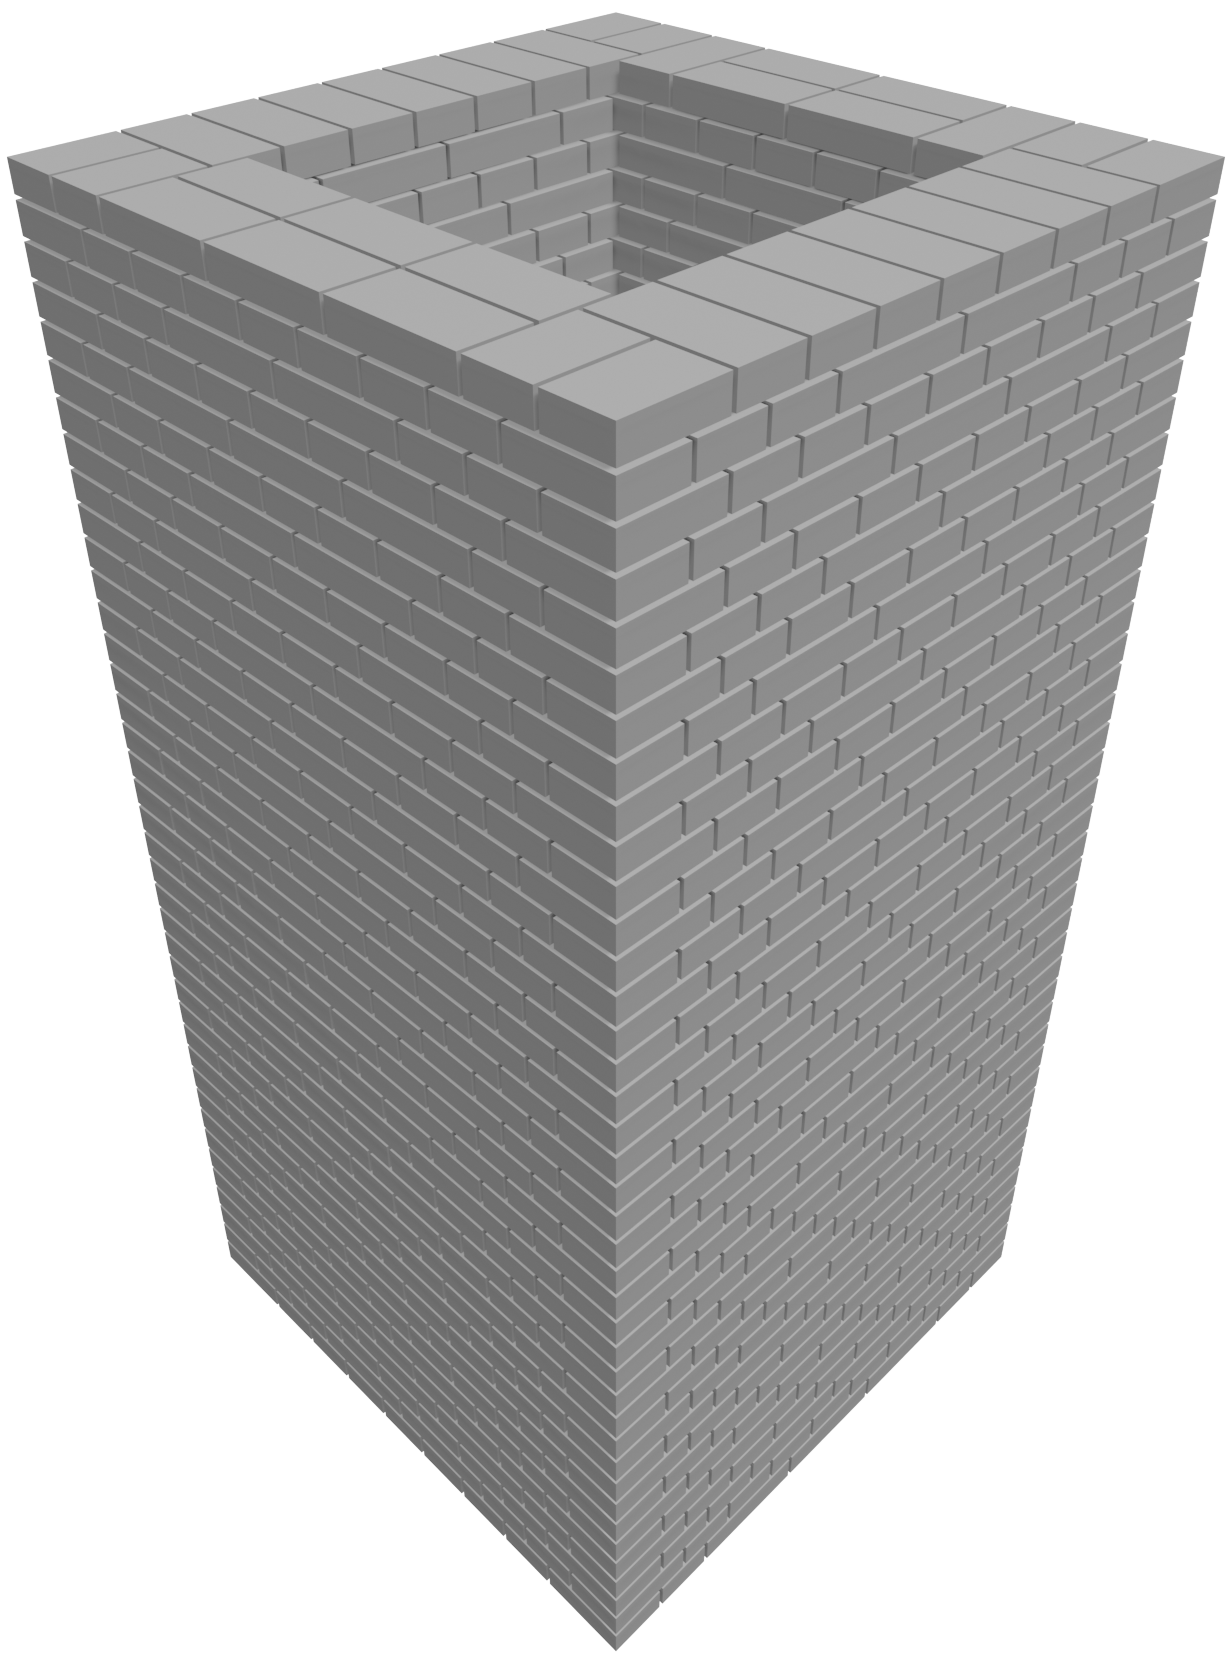
\includegraphics[width=\columnwidth]{fig/scenario1_render_crossbond.png}
      \caption{Kreuzverband mit 1360 Bausteinen.}\label{fig:poc:render_crossbond}
    \end{subfigure}
    \hfill
    \begin{subfigure}[b]{0.3\columnwidth}
      \includegraphics[width=\columnwidth]{fig/scenario1_render_läuferverband50.png}
      \caption{Läuferverband mit 720 Bausteinen.}\label{fig:poc:render_laeuferverband50}
    \end{subfigure}
    \hfill
    \begin{subfigure}[b]{0.3\columnwidth}
      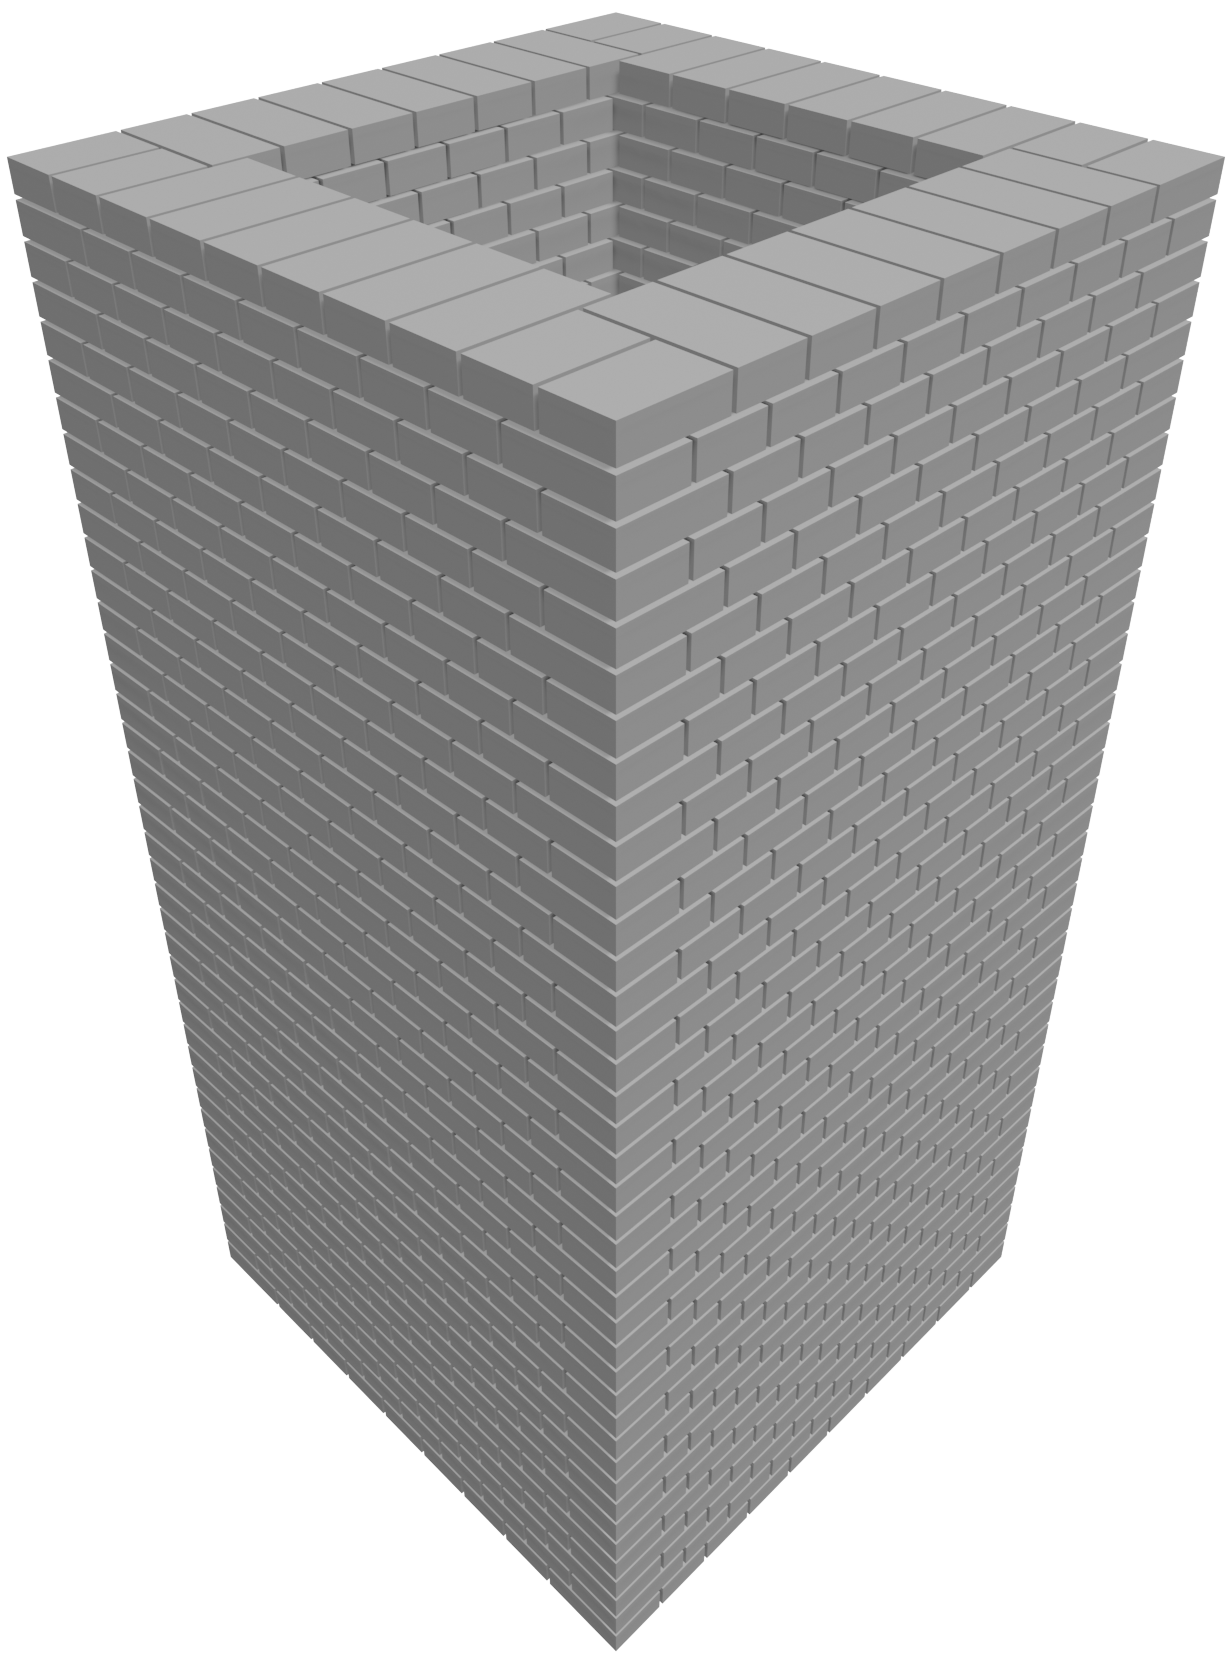
\includegraphics[width=\columnwidth]{fig/scenario1_render_headbond.png}
      \caption{Kopfverband mit 1360 Bausteinen.}\label{fig:poc:render_headbond}
    \end{subfigure}
    \caption{Ergebnisse des Wall Detailings mit unterschiedlichen Verbänden.}\label{fig:poc:result_scenario1}
\end{figure}

\subsection{Szenario LEGO Klemmbausteine}\label{poc:scenario2}
Die Modellierung dieses Szenarios war aufgrund der Fenster und Türen ein wenig anspruchsvoller.
Das dafür vorgesehene Vorgehen innerhalb der BIM Erweiterung für Blender ist zunächst etwas versteckt.
Zumindest ist das Hinzufügen neuer Tür- und Fensterarten ist der Definition neuer Wandarten sehr ähnlich.
Das finale Modell ist in Abbildung~\ref{fig:poc:scenario2 modell} zu sehen.
In Kapiteln~\ref{concept:openings} und~\ref{real:openings} wurde bereits aufgeführt, wie Öffnungen aus dem Modell extrahiert und als Teil des Wall-Detailings berücksichtigt werden.
Das in Abbildung~\ref{fig:poc:scenario2_ergebnis} zu sehende Ergebnis zeigt die korrekte Umsetzung der Fenster und Türbereiche.
In Kapitel~\ref{basics:Mauerwerksverband} wurde schon die sogenannte Stumpfstoßtechnik angesprochen.
Dabei werden Anker dazu verwendet zwei Wandstücke miteinander zu verbinden, ohne dass diese verzahnt werden müssen.
Da es für T- und X-Kreuzungen selbst bei Wandstücken mit gleichem Modul, Raster und Verband zu einer Vielzahl unterschiedlicher Kreuzungssituationen kommen kann, wurde zunächst darauf verzichtet dies in den Kreuzungslegeplänen der verschiedenen Verbände einzupflegen, obwohl das mit dem erarbeiteten Konzept möglich wäre.
Stattdessen wird sich an diesen Stellen auf die Stumpfstoßtechnik berufen und das algorithmische Auflösen der Kreuzungsbereiche als weiterführendes Konzept betrachtet.
Wie bereits mehrfach in Kapitel~\ref{related:planungsvorgehen} erwähnt, könnten dazu \glqq{}intelligente\grqq{} beziehungsweise lernende Algorithmen eingesetzt werden.

\begin{figure}[htb]
  \begin{subfigure}[b]{0.49\columnwidth}
    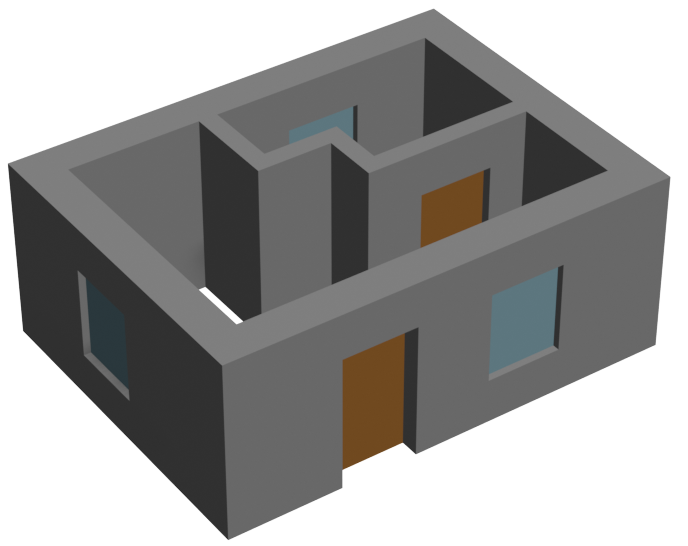
\includegraphics[width=\columnwidth]{fig/scenario2_rendering_input.png}
    \caption{Gebäudemodell.}\label{fig:poc:scenario2 modell}
  \end{subfigure}
  \hfill
  \begin{subfigure}[b]{0.49\columnwidth}
    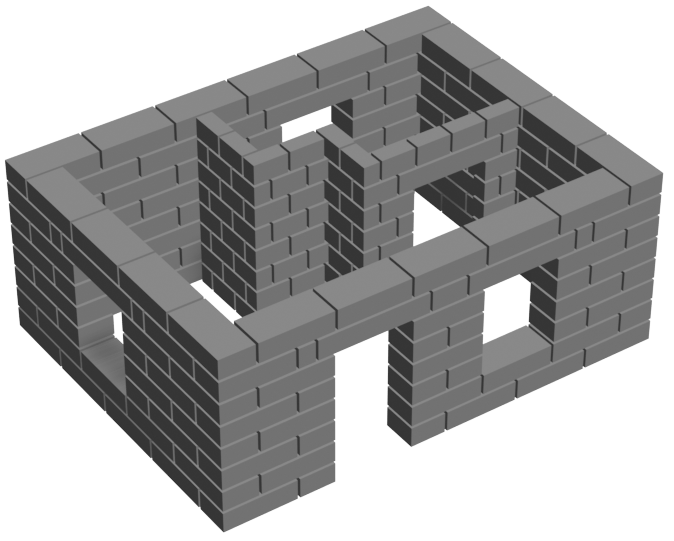
\includegraphics[width=\columnwidth]{fig/scenario2_render.png}
    \caption{Ergebnis mit 223 Bausteinen.}\label{fig:poc:scenario2_ergebnis}
  \end{subfigure}
\caption{Eingabemodell und Ergebnis für das Szenario LEGO Klemmbausteine.}\label{fig:poc:result_scenario2}
\end{figure}

\subsection{Szenario Fabrikgebäude}\label{poc:scenario3}
Dieses Szenario besteht aus insgesamt 36 einzelnen Wandstücken.
Es gibt drei unterschiedliche Wandtypen.
Vom ersten Typ, der eine 0.125 Meter dicke Wand aus 1 DF Steinen und halbversetztem Läuferverband vorschreibt, gibt es 20 Stück.
Wände des zweiten Typs sind 0.25 Meter dick und werden im Kreuzverband mit 2 DF Steinen realisiert.
Davon existieren 12 Stück.
Für den Sockel des Kamins wurde ein eigener 0.5 Meter dicker Wandtyp definiert.
Der Sockel soll mit Steinen im 16 DF Format und unter Anwendung des Kopfverbands erbaut werden.
Darum gibt es von diesem Typ lediglich 4 Wände, auf welchen der eigentliche Kamin ruht.
Außerdem wurden insgesamt 45 Fenster und 13 Türen an den Wänden angebracht.
Um einen Dachgiebel anzudeuten, wurden niedrige und kürzer werdende Wandstücke auf den Mittelteil und dem seitlichen Anbau des Gebäudes gesetzt.
Diese kleineren Wandstücke werden im Kombinationsschritt des Wall Detailings mit den großen darunterliegenden Wandstücken verschmolzen (siehe Abschnitt~\ref{real:combination}).
Darum werden aus den 12 Wandstücken des zweiten Typs 4 und aus den 20 Wandstücken des ersten Typs 12.
Dieser Schritt stellt zusammen mit dem Schritt des Findens und Lösens der Eckbereiche (siehe Abschnitt~\ref{real:find_and_solve}) den zeitaufwendigsten dar.
Der Aufwand diese beiden Schritte zu berechnen verhält sich jeweils quadratisch zur Anzahl der einzelnen Schichten der beteiligten Wandstücke.
Die Zeit zur Berechnung der konkreten Bausteine ist linear zur Anzahl der notwendigen Ziegel.
In einem früheren Implementierungsversuch hatte das Finden von Nachbarschaftsbeziehungen zwischen Bausteinen ebenfalls eine quadratische Laufzeit in Abhängigkeit zur Anzahl der Bausteine und der Größe des angegebenen Rasters.
Später konnte dieses Vorgehen aber optimiert und ebenfalls eine lineare Laufzeit erreicht werden.
Ein ähnlicher Ansatz könnte für das Kombinieren und Lösen von Eckbereichen womöglich auch anwendbar sein.

\begin{figure}[bt]
  \centering
  \includegraphics[width=0.9\columnwidth]{fig/scenario3_output_render2.png}
  \caption{Ausschnitt des Ergebnisses von Szenario Fabrikgebäude mit 40409 Bausteinen.}\label{fig:poc:scenario3}
\end{figure}

\section{Regelbasierte Bauplandeduktion aus einem Bauplanentwurf}
Mithilfe der in Kapitel~\ref{basics:ontologie} eingeführten Technologie einer Ontologie und der konkreten Umsetzung der Baustein- und Regeldefinitionen nach dem Konzept aus Abschnitt~\ref{concept:regelbasierte_bauplandeduktion} 
konnte der resultierende Bauplanentwurf des Modells dieser Fallstudie in die dafür erstellte Ontologie eingepflegt werden.
Das Konzept der Regeln wurde in dieser Fallstudie anhand der dafür erstellten \textit{RuleDependsOnBottomNeighbor} Regel getestet.
Diese soll alle nach unten benachbarten Bausteine eines Bausteins in dessen \textit{dependsOn} Objekteigenschaft übertragen, sodass nur diejenigen Bausteine der Klasse \textit{NextBrick} zugeordnet werden können, die keine Individuen der Klasse \textit{PlaceableBrick} als untere Nachbarn besitzen.
Dafür wurde für das Regel-Individuum über die Dateneigenschaft \textit{holdPropertyByName} der Name der Ziel-Objekteigenschaft \textit{hasBottomNeighbor} festgelegt.
Über die Objekteigenschaft \textit{applyObjectPropertyTo} wurde schließlich auf das dafür erstelle \textit{ObjectPropertyHolder}-Individuum \textit{dependsOnObjectPropertyHolder} verwiesen.
Dieses wiederum hält lediglich den Namen der Objekteigenschaft \textit{dependsOn}.
Mit diesen Informationen kann nun während der Befüllung der Ontologie mit konkreten Bausteinen deren \textit{dependsOn} Objekteigenschaften mit den Einträgen aus deren unteren Nachbarn gleichgesetzt werden.

Im Anschluss wurde durch wiederholtes Ausführen eines Reasoners und Auswählen einer zufälligen nächsten Instanz der Klasse \textit{NextBrick} ein Bauplan erstellt, der die in Abbildung~\ref{fig:scenarios:Scenario4 Experiment} gezeigte Wand von unten nach oben erbaut.
In Abbildung~\ref{fig:poc:result_scenario4} sind drei Zwischenergebnisse dieses Vorgehens zu sehen.
Insgesamt enthält die Wand 28 Steine.

\begin{figure}[htb]
  \begin{subfigure}[b]{0.3\columnwidth}
    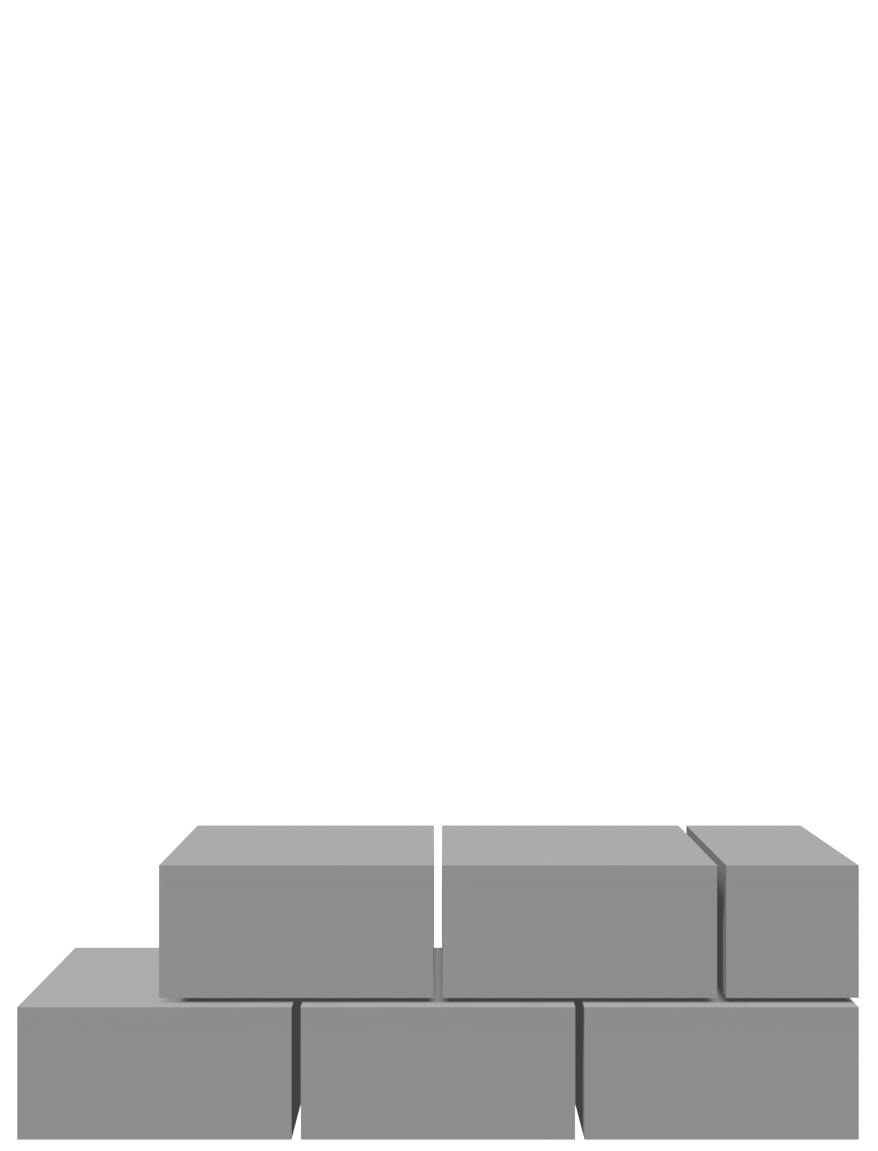
\includegraphics[width=\columnwidth]{fig/scenario4_output_6_render.png}
    \caption{Ergebnis nach 6 Schritten.}
  \end{subfigure}
  \hfill
  \begin{subfigure}[b]{0.3\columnwidth}
    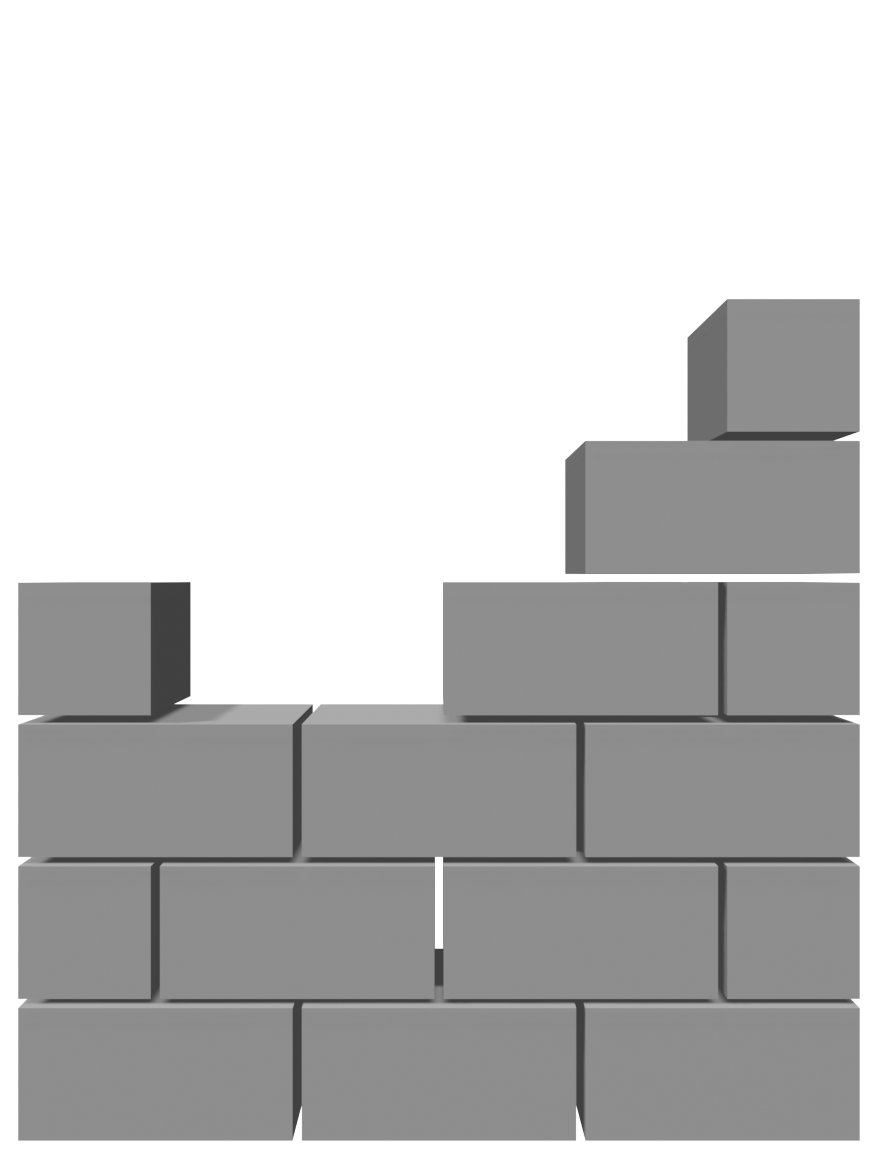
\includegraphics[width=\columnwidth]{fig/scenario4_output_15_render.png}
    \caption{Nach 15 Schritten.}
  \end{subfigure}
  \hfill
  \begin{subfigure}[b]{0.3\columnwidth}
    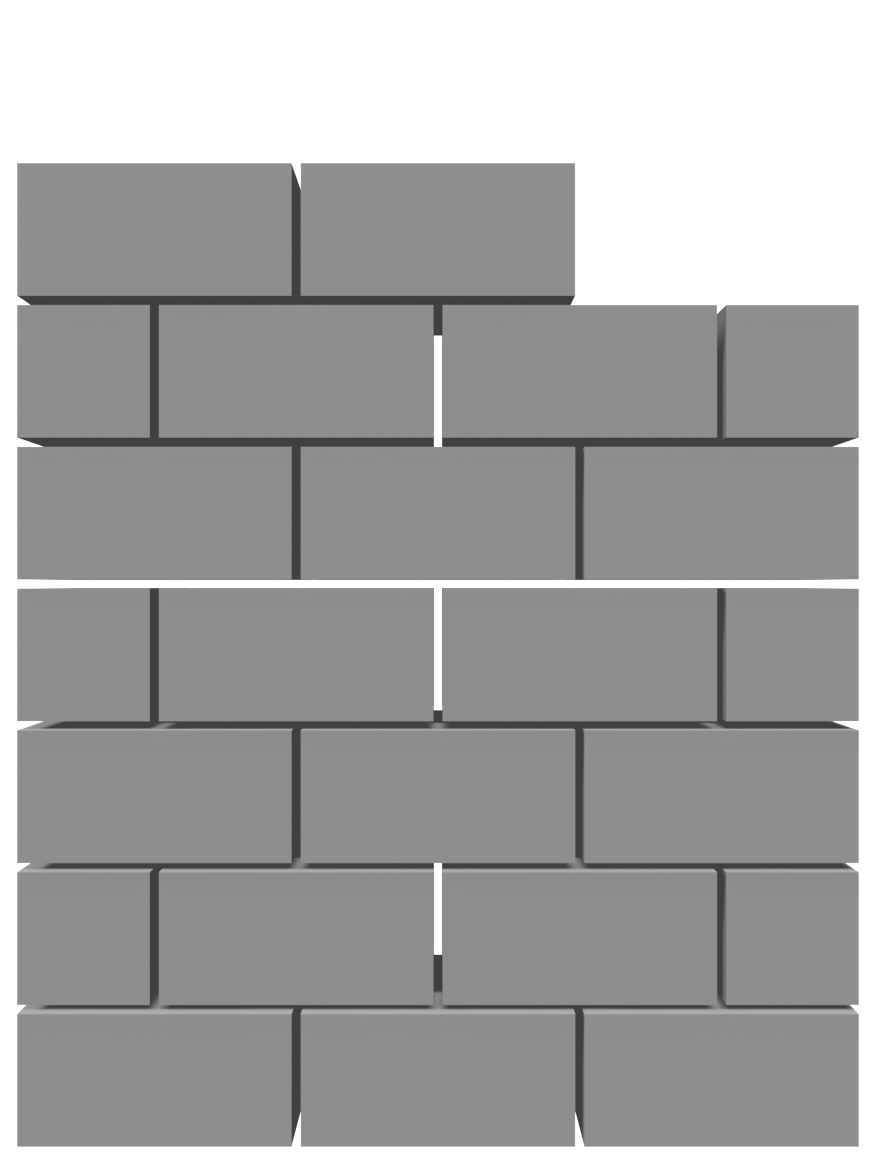
\includegraphics[width=\columnwidth]{fig/scenario4_output_23_render.png}
    \caption{Nach 23 Schritten.}
  \end{subfigure}
  \caption{Schrittweises Platzieren eines gefundenen NextBrick.}\label{fig:poc:result_scenario4}
\end{figure}